%% LyX 2.2.1 created this file.  For more info, see http://www.lyx.org/.
%% Do not edit unless you really know what you are doing.
\documentclass[10pt]{beamer}\usepackage[]{graphicx}\usepackage[]{color}
%% maxwidth is the original width if it is less than linewidth
%% otherwise use linewidth (to make sure the graphics do not exceed the margin)
\makeatletter
\def\maxwidth{ %
  \ifdim\Gin@nat@width>\linewidth
    \linewidth
  \else
    \Gin@nat@width
  \fi
}
\makeatother

\definecolor{fgcolor}{rgb}{0.345, 0.345, 0.345}
\newcommand{\hlnum}[1]{\textcolor[rgb]{0.686,0.059,0.569}{#1}}%
\newcommand{\hlstr}[1]{\textcolor[rgb]{0.192,0.494,0.8}{#1}}%
\newcommand{\hlcom}[1]{\textcolor[rgb]{0.678,0.584,0.686}{\textit{#1}}}%
\newcommand{\hlopt}[1]{\textcolor[rgb]{0,0,0}{#1}}%
\newcommand{\hlstd}[1]{\textcolor[rgb]{0.345,0.345,0.345}{#1}}%
\newcommand{\hlkwa}[1]{\textcolor[rgb]{0.161,0.373,0.58}{\textbf{#1}}}%
\newcommand{\hlkwb}[1]{\textcolor[rgb]{0.69,0.353,0.396}{#1}}%
\newcommand{\hlkwc}[1]{\textcolor[rgb]{0.333,0.667,0.333}{#1}}%
\newcommand{\hlkwd}[1]{\textcolor[rgb]{0.737,0.353,0.396}{\textbf{#1}}}%
\let\hlipl\hlkwb

\usepackage{framed}
\makeatletter
\newenvironment{kframe}{%
 \def\at@end@of@kframe{}%
 \ifinner\ifhmode%
  \def\at@end@of@kframe{\end{minipage}}%
  \begin{minipage}{\columnwidth}%
 \fi\fi%
 \def\FrameCommand##1{\hskip\@totalleftmargin \hskip-\fboxsep
 \colorbox{shadecolor}{##1}\hskip-\fboxsep
     % There is no \\@totalrightmargin, so:
     \hskip-\linewidth \hskip-\@totalleftmargin \hskip\columnwidth}%
 \MakeFramed {\advance\hsize-\width
   \@totalleftmargin\z@ \linewidth\hsize
   \@setminipage}}%
 {\par\unskip\endMakeFramed%
 \at@end@of@kframe}
\makeatother

\definecolor{shadecolor}{rgb}{.97, .97, .97}
\definecolor{messagecolor}{rgb}{0, 0, 0}
\definecolor{warningcolor}{rgb}{1, 0, 1}
\definecolor{errorcolor}{rgb}{1, 0, 0}
\newenvironment{knitrout}{}{} % an empty environment to be redefined in TeX

\usepackage{alltt}
\usepackage[T1]{fontenc}
\setcounter{secnumdepth}{3}
\setcounter{tocdepth}{3}
\usepackage{url}
\ifx\hypersetup\undefined
  \AtBeginDocument{%
    \hypersetup{unicode=true,pdfusetitle,
 bookmarks=true,bookmarksnumbered=false,bookmarksopen=false,
 breaklinks=false,pdfborder={0 0 0},pdfborderstyle={},backref=false,colorlinks=false}
  }
\else
  \hypersetup{unicode=true,pdfusetitle,
 bookmarks=true,bookmarksnumbered=false,bookmarksopen=false,
 breaklinks=false,pdfborder={0 0 0},pdfborderstyle={},backref=false,colorlinks=false}
\fi
\usepackage{breakurl}

\makeatletter

%%%%%%%%%%%%%%%%%%%%%%%%%%%%%% LyX specific LaTeX commands.
\providecommand{\LyX}{\texorpdfstring%
  {L\kern-.1667em\lower.25em\hbox{Y}\kern-.125emX\@}
  {LyX}}

%%%%%%%%%%%%%%%%%%%%%%%%%%%%%% Textclass specific LaTeX commands.
 % this default might be overridden by plain title style
 \newcommand\makebeamertitle{\frame{\maketitle}}%
 % (ERT) argument for the TOC
 \AtBeginDocument{%
   \let\origtableofcontents=\tableofcontents
   \def\tableofcontents{\@ifnextchar[{\origtableofcontents}{\gobbletableofcontents}}
   \def\gobbletableofcontents#1{\origtableofcontents}
 }

%%%%%%%%%%%%%%%%%%%%%%%%%%%%%% User specified LaTeX commands.
%\usetheme{PaloAlto}
\usepackage{subcaption}

\makeatother
\IfFileExists{upquote.sty}{\usepackage{upquote}}{}
\begin{document}


\title[knitr, Beamer, and FragileFrame]{Hierarchical Latent Space Models\\ for Multiplex Social Network Analysis}

\author{Alex Loewi}%\thanks{I thank Richard E. Goldberg for providing this demo.}}
\makebeamertitle
\begin{frame}{Motivation}

\begin{itemize}
\item I have multiplex data -- five edge types (``layers'') over 80 nodes
\begin{enumerate}
\item Discuss Academics
\item Discuss Behavior
\item Talk Socially
\item Talk Frequently
\item Helpful
\end{enumerate}
\item I want to understand this data in as many ways as possible BUT
\item Models are rare
\item The data is complicated
\item Visualization is hard
\end{itemize}

% \begin{itemize}
% \item The \textbf{knitr}\textbf{\emph{ }}package allows you to embed R code
% and figures in \LaTeX{} documents
% 
% \begin{itemize}
% \item It has functionality similar to Sweave but looks nicer and gives you
% more control
% \end{itemize}
% \item If you already have Sweave working in \LyX{}, getting \textbf{knitr}
% to work is trivial
% 
% \begin{enumerate}
% \item Install the \textbf{knitr} package in \emph{R}
% \item Read \url{https://yihui.name/knitr/demo/lyx/}
% \end{enumerate}
% \item If you use Sweave or \textbf{knitr} with Beamer in \LyX{}, you must
% use the\emph{ FragileFrame} environment for the frames that contain
% R code chunks. Let's see if \textbf{knitr} works with Beamer in this
% small demo. 
% \end{itemize}

\end{frame}

\begin{frame}{Visualizing Multigraphs}
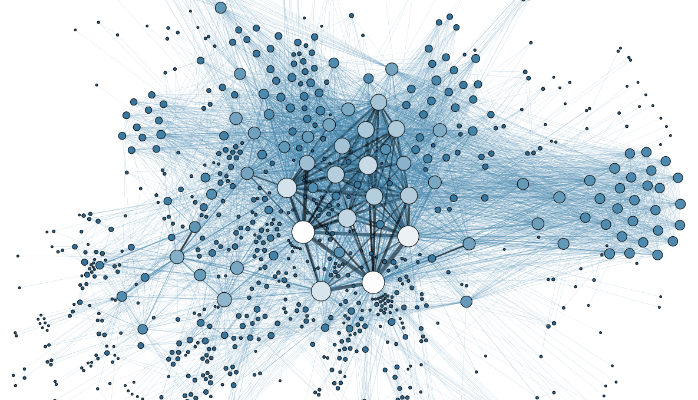
\includegraphics[width=\textwidth]{force_layout.png}
\end{frame}

\begin{frame}{Visualizing Multigraphs}
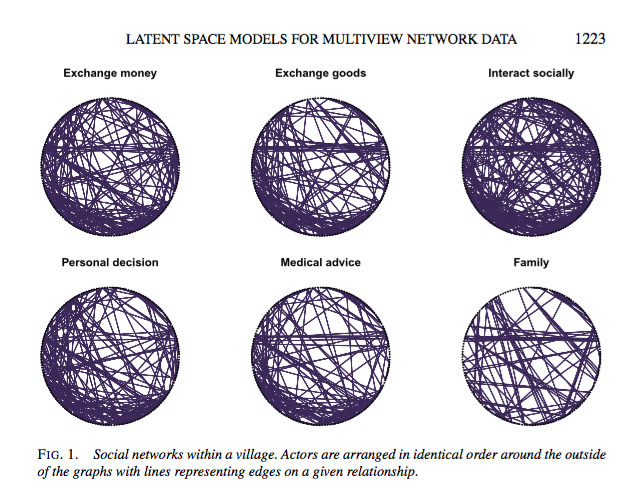
\includegraphics[width=\textwidth]{mvlsm_layouts.png}
\end{frame}

\begin{frame}{Visualizing Multigraphs}
\begin{center}
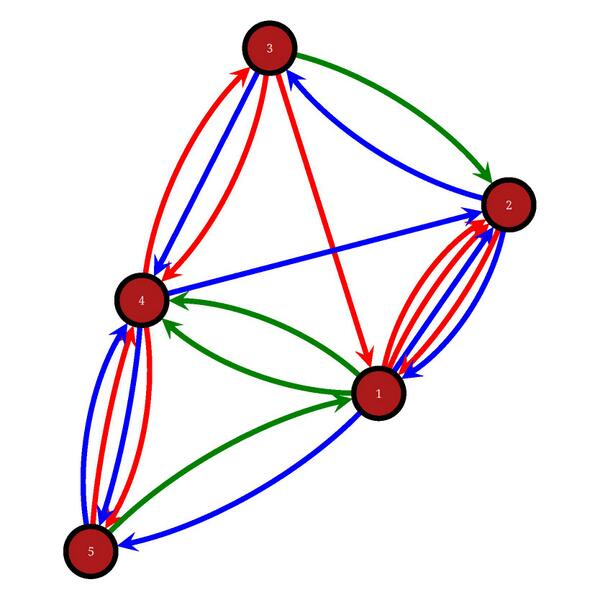
\includegraphics[width=.5\textwidth]{multigraph.jpg}
\end{center}
\end{frame}

\begin{frame}{Visualizing Multigraphs}
\begin{itemize}
\item Graph \textbf{layouts} require node positions to be \textbf{flexible}
\item Graph \textbf{comparisons} require node positions to be \textbf{stable}
\item Is there a way to manually tune between the extremes?
\end{itemize}
\end{frame}


\begin{frame}{A Proposal}
Hierarchical models are tunable in this way
\begin{enumerate}
\item Have a single set of ``base'' positions for the nodes
\item Positions for a given layer are perturbations from that base position

\[
\prod_k \prod_{ij} \sigma_{ijk}^{y_{ijk}}(1- \sigma_{ijk})^{1-y_{ijk}}
\]

\[
\sigma_{ijk} = \text{logit}^{-1}(\alpha_k - d(z_{ik}, z_{jk}))
\]

\[
z_{ik} = b_i + \epsilon_{ik}
\]

\item Regularizing these perturbations allows for tuning
\item (and a lasso penalty grouped layer-wise could reduce the dimensionality)
\end{enumerate}


\end{frame}


\begin{frame}{STAN}
\begin{center}
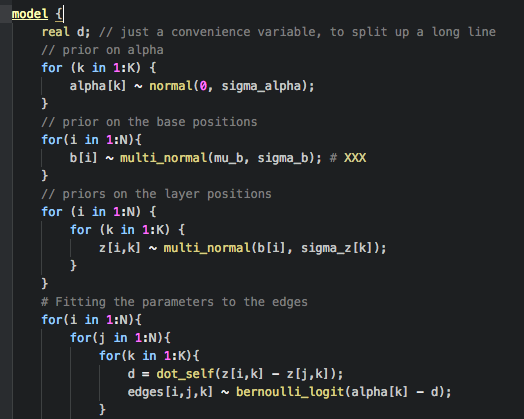
\includegraphics[width=.8\textwidth]{stan.png}
\end{center}
\end{frame}


\begin{frame}{The Test}
\begin{center}
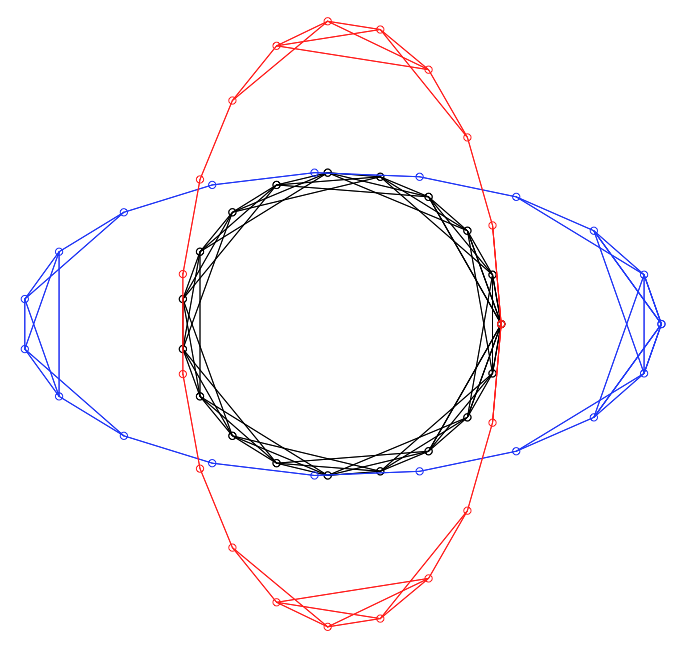
\includegraphics[width=.8\textwidth]{hlsm_sim.png}
\end{center}
\end{frame}


\begin{frame}{Some Results}
% \begin{center}
% % DO A DOUBLE PLOT SIDE BY SIDE
% 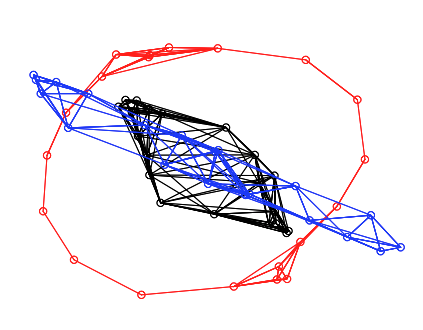
\includegraphics[width=.8\textwidth]{hlsm_20k.png}
% \end{center}

\begin{figure}[ht]
  \centering
  \begin{subfigure}[b]{0.5\linewidth}
    \centering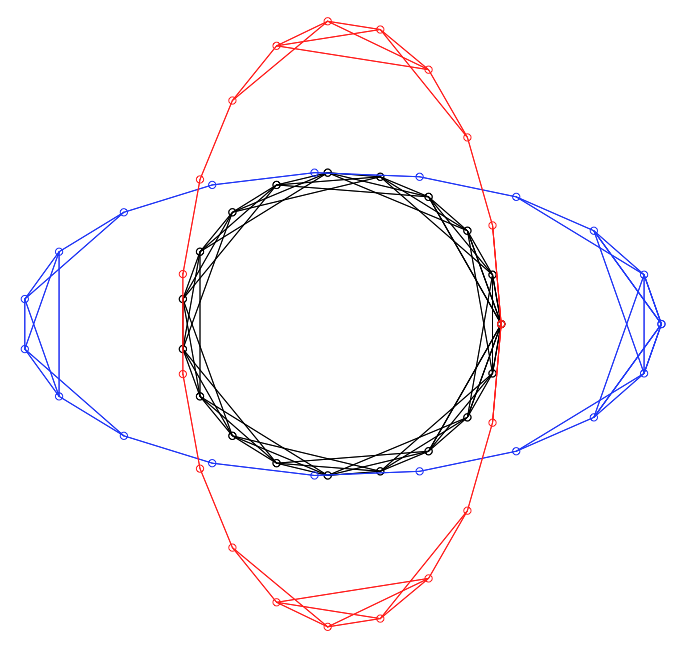
\includegraphics[width=120pt]{hlsm_sim.png}
    \caption{\label{fig:hlsm_sim}}
  \end{subfigure}%
  \begin{subfigure}[b]{0.5\linewidth}
    \centering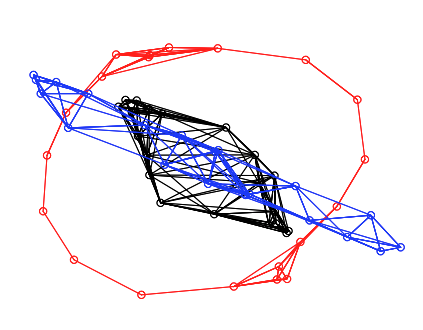
\includegraphics[width=120pt]{hlsm_20k.png}
    \caption{\label{fig:hlsm_20k}}
  \end{subfigure}
  \caption{Original, and Estimates}
\end{figure}

\end{frame}


\section{MVLSM}
\begin{frame}{A Recent Model}


\includegraphics[width=\textwidth]{mvlsm.png}

% OK, let's get started with just some text:
% 
% <<echo=FALSE,results='hide'>>=
% # some setup
% options(width=60)  # make the printing fit on the page
% set.seed(1121)   # make the results repeatable
% @
% 
% <<>>= 
% # create some random numbers
% (x=rnorm(20))  
% mean(x);var(x)  
% @
% 
% BTW, the first element of \texttt{x} is x[1]. (Did you notice
% the use of\texttt{ \textbackslash{}Sexpr\{\}}?)

\end{frame}


\begin{frame}{A Recent Model}

Their model:
\begin{enumerate}
\item Separate set of latent variables for each layer
\item Correlations between layers
\end{enumerate}
Intuition: An edge could exist because its nodes are close, OR because its nodes are close in a correlated layer. However ...
\vspace{.5cm}
%\begin{displayquote}

\begin{center}
{\fontfamily{times}\selectfont
`` ... our current model is way too flexible.''
}
\end{center}
\begin{flushright}
-- The Authors \:\:\:\:\:
\end{flushright}
%\end{displayquote}

\end{frame}


\begin{frame}{Advantages}
\begin{itemize}
\item Models are rare
\item The data is complicated 
\item Visualization is hard 
\item (Model too flexible)
\end{itemize}
\end{frame}

\begin{frame}{Advantages}
\begin{itemize}
\item Models are rare         \hfill -- here's another one!
\item The data is complicated 
\item Visualization is hard   
\item (Model too flexible)    
\end{itemize}
\end{frame}

\begin{frame}{Advantages}
\begin{itemize}
\item Models are rare         \hfill -- here's another one!
\item The data is complicated \hfill -- data reduction!
\item Visualization is hard   
\item (Model too flexible)    
\end{itemize}
\end{frame}

\begin{frame}{Advantages}
\begin{itemize}
\item Models are rare         \hfill -- here's another one!
\item The data is complicated \hfill -- data reduction!
\item Visualization is hard   \hfill -- make layers comparable!
\item (Model too flexible)    
\end{itemize}
\end{frame}

\begin{frame}{Advantages}
\begin{itemize}
\item Models are rare         \hfill -- here's another one!
\item The data is complicated \hfill -- data reduction!
\item Visualization is hard   \hfill -- make layers comparable!
\item (Model too flexible)    \hfill -- this one isn't!
\end{itemize}
\end{frame}

\begin{frame}{Next Steps}
\textbf{A Full To-Do List}
\begin{itemize}
\item More test cases
\begin{enumerate}
\item Dimensionality reduction,
\item Visual comparability, 
\item More complex graphs
\end{enumerate}
\item Better theory around fitting
\item ... so as to find better \textit{methods} for fitting
\item Way to find a good starting point (use normal LSMs?)
\end{itemize}
\vspace{1cm}
\textbf{Issues already encountered -- }
\begin{itemize}
\item The intercepts are being difficult
\item 20k iterations take half an hour, fewer don't burn in
\item ...
\end{itemize}
\end{frame}


\begin{frame}{Some Results}
% \begin{center}
% % DO A DOUBLE PLOT SIDE BY SIDE
% 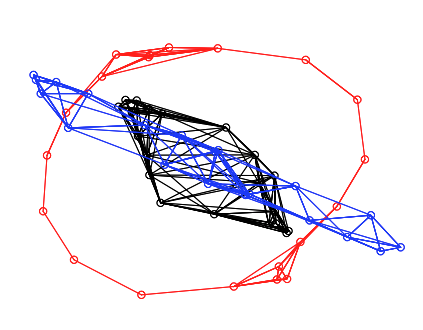
\includegraphics[width=.8\textwidth]{hlsm_20k.png}
% \end{center}

\begin{figure}[ht]
  \centering
  \begin{subfigure}[b]{0.5\linewidth}
    \centering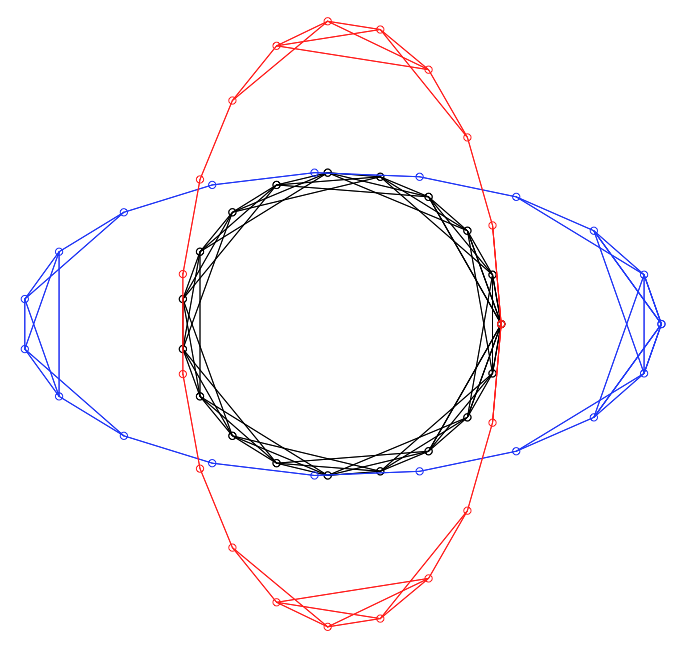
\includegraphics[width=120pt]{hlsm_sim.png}
    \caption{\label{fig:hlsm_sim}}
  \end{subfigure}%
  \begin{subfigure}[b]{0.5\linewidth}
    \centering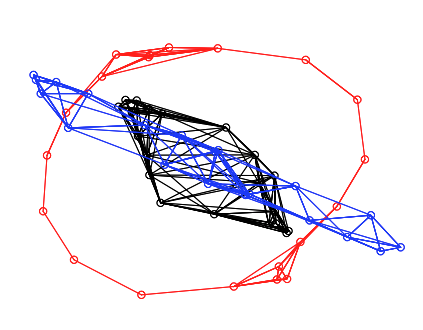
\includegraphics[width=120pt]{hlsm_20k.png}
    \caption{\label{fig:hlsm_20k}}
  \end{subfigure}
  \caption{Original, and Estimates}
\end{figure}

\end{frame}


\begin{frame}{Preparing Your Next Presentation}
\begin{figure}[ht]
  \centering
  \begin{subfigure}[b]{0.3\linewidth}
    \centering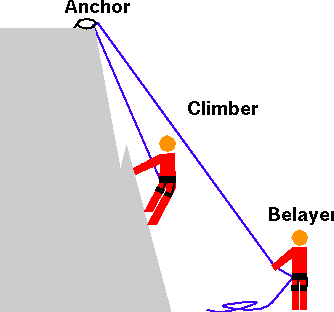
\includegraphics[width=100pt]{climbers.png}
    \caption{\label{fig:climbers}}
  \end{subfigure}%
  \hspace{1cm}
  \begin{subfigure}[b]{0.15\linewidth}
    \centering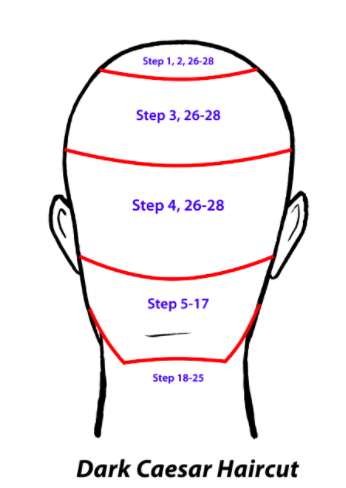
\includegraphics[width=70pt]{haircut.png}
    \caption{\label{fig:haircut}}
  \end{subfigure}
    \begin{subfigure}[b]{0.7\linewidth}
    \centering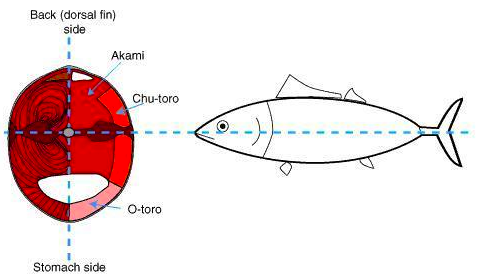
\includegraphics[width=150pt]{tuna.png}
    \caption{\label{fig:tuna}}
  \end{subfigure}
  \caption{Images that Evidently Resemble My Graphics}
\end{figure}
\end{frame}



% \section{Second Test}
% \begin{frame}[fragile]{Second Test}
% 
% Text is nice but let's see what happens if we make a couple of plots
% in our chunk:
% 
% <<boring-plots,fig.width=4,fig.height=4,out.width='.45\\linewidth'>>=
% par(las=1,mar=c(4,4,.1,.1))  # tick labels direction
% boxplot(x) 
% hist(x,main='',col="blue",probability=TRUE) 
% lines(density(x),col="red")
% @
% \end{frame}


\end{document}
